
\chapter{Linear independence}

\index{linear independence}

One of the deepest and most central concepts in linear algebra -- in fact, if I
were to make a top ten ranking, this one might just make \#1 -- is that of
\textbf{linear independence}. It's not about mechanical computations, but
conceptual truths. Learn this chapter well. 

\section{The Domino Game}
\index{the Domino Game}

I've thought long and hard about the best way to teach the material in this
chapter, and I've come up with a game. I call it ``the Domino Game.'' Here are
the rules:

\begin{framed}
\begin{compactenum}
\item You are given one or more yellow\footnotemark ``starter dominoes.''
\item The object of the game is to build the white ``goal domino'' from these
starter dominoes.
\item You can ``use'' any number of each starter domino (even a fraction, even
negative), and add them together (left sides add together, and right sides add
together).
\item You \textit{cannot} use only one side of a domino.
\item You \textit{cannot} turn a domino around so the left side and right
sides flip.
\end{compactenum}
\end{framed}

\footnotetext{Gray, actually, since I made this a black and white book to keep costs down.}

Example. Suppose your starter dominoes are:

\begin{center}
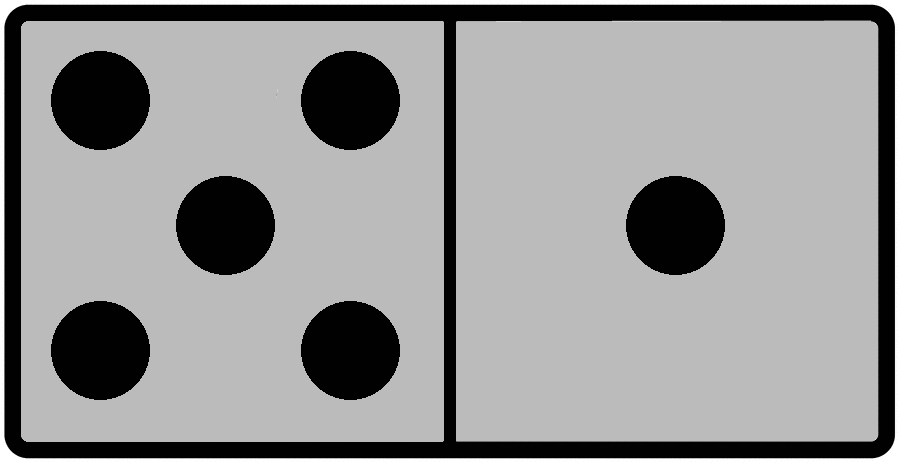
\includegraphics[width=0.3\textwidth]{gray5_1.png}
\hspace{.3in}
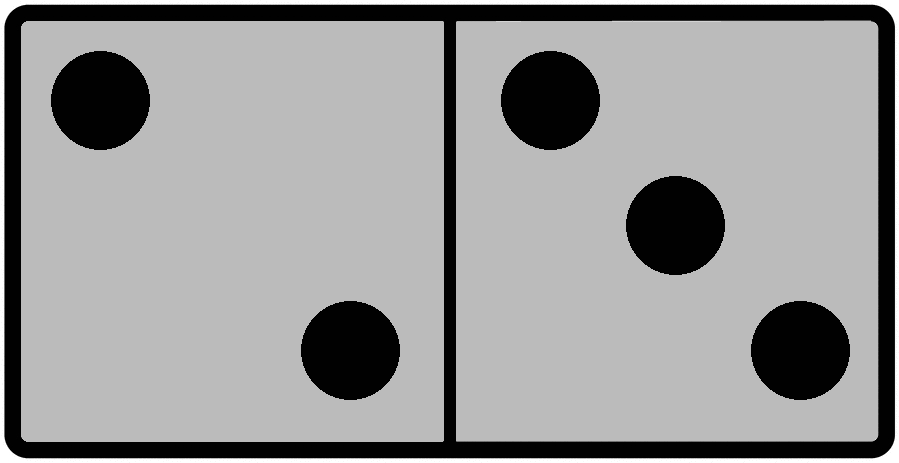
\includegraphics[width=0.3\textwidth]{gray2_3.png}
\end{center}

and your goal domino is:
\begin{center}
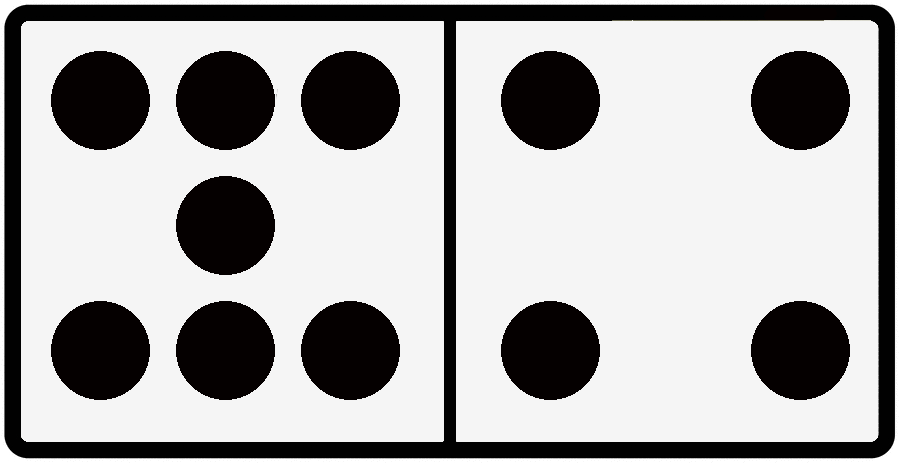
\includegraphics[width=0.3\textwidth]{white7_4.png}
\end{center}

A solution would be ``\textbf{one} and \textbf{one}.'' This means that you'll
take \textit{one} copy of the first starter domino, and \textit{one} copy of
the second, and add them together.

\begin{center}
{\LARGE Solution: \textbf{1 \& 1}}

1 \raisebox{-0.3\height}{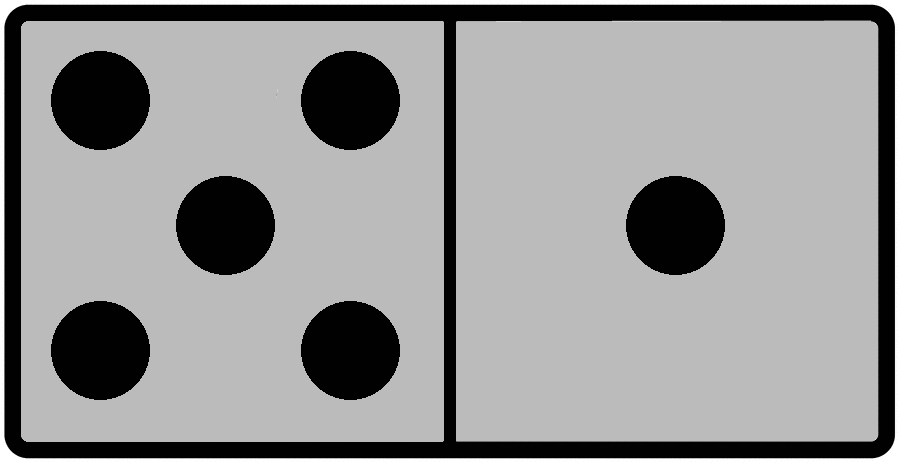
\includegraphics[width=0.1\textwidth]{gray5_1.png}} \ \& \
1 \raisebox{-0.3\height}{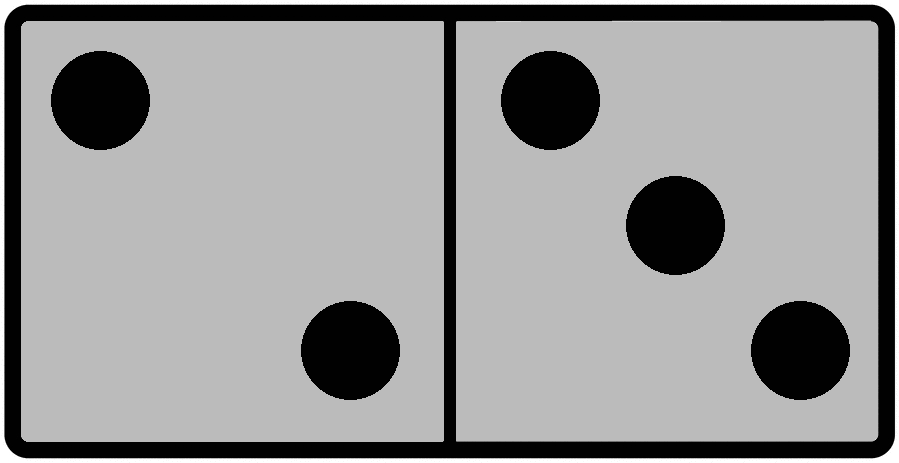
\includegraphics[width=0.1\textwidth]{gray2_3.png}} \ = \
\raisebox{-0.3\height}{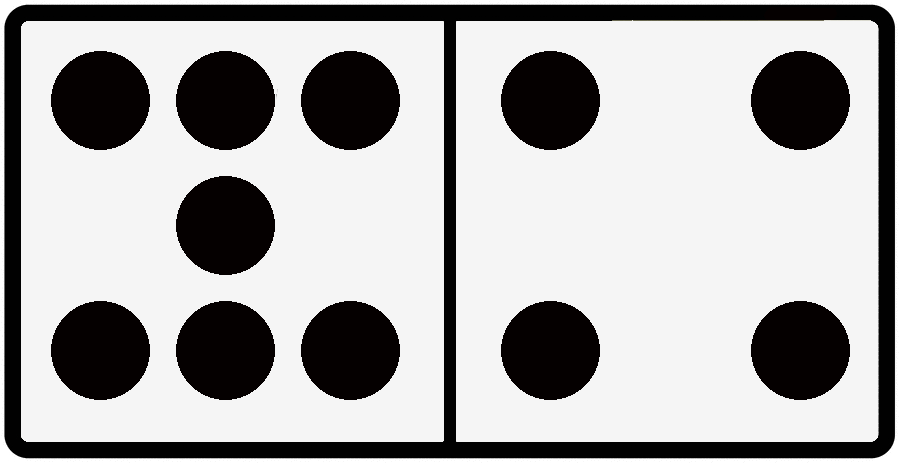
\includegraphics[width=0.1\textwidth]{white7_4.png}} \quad
\end{center}

Stare carefully at that until you master how it works; the rest of this chapter
will be a complete waste of time if this operation is not fully grasped. Adding
domino 5--1 to 2--3 means adding the left sides together, and separately adding
the right sides together, to produce a new domino 7--4 (since $5+2=7$ and
$1+3=4$).

\subsection{Actually do this}

All right, let's test your skillz. I want you to \textit{actually} work out the
answers to the following Domino Game puzzles on your own. There are six of
them, so it might take you a while (perhaps as long as 6 minutes). But it's
vital to cement your understanding of how this works...\textit{and} to set up
the crucial punchline later on in this chapter.

Answers to each puzzle are given at the end of the chapter. Maybe your answers
will not be the same as mine...or maybe they will? That itself is actually a
very important question we'll consider in a few minutes.

Enough preamble. Go!

\begin{enumerate}
\itemsep2em

\label{startDominoPuzzes}
\item Starter dominoes:
\hspace{.3in}
\raisebox{-0.3\height}{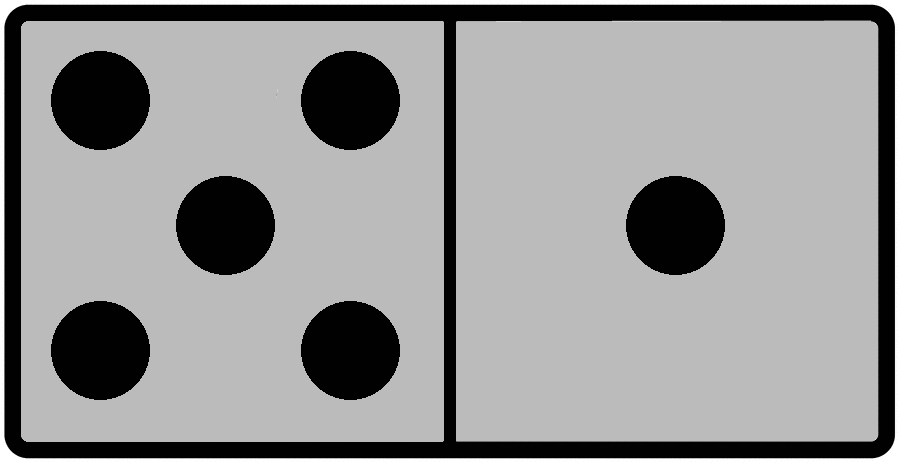
\includegraphics[width=0.2\textwidth]{gray5_1.png}}
\hspace{.1in}
\raisebox{-0.3\height}{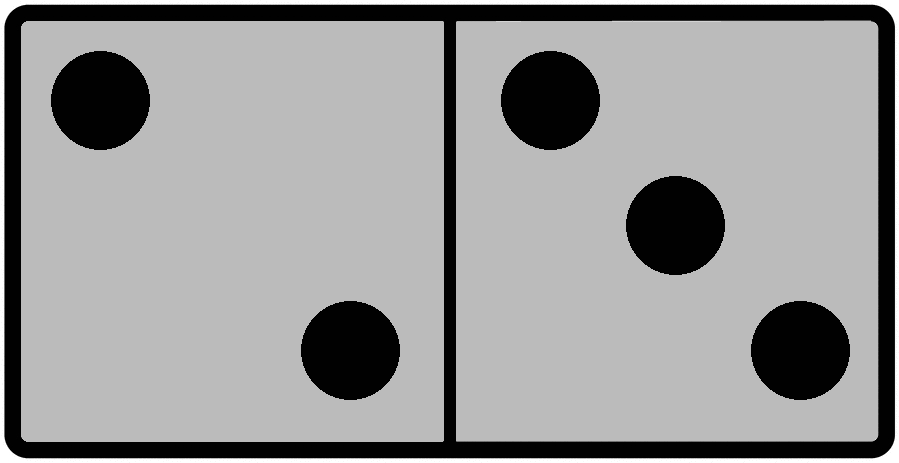
\includegraphics[width=0.2\textwidth]{gray2_3.png}}

Goal domino:
\hspace{1.1in}
\raisebox{-0.3\height}{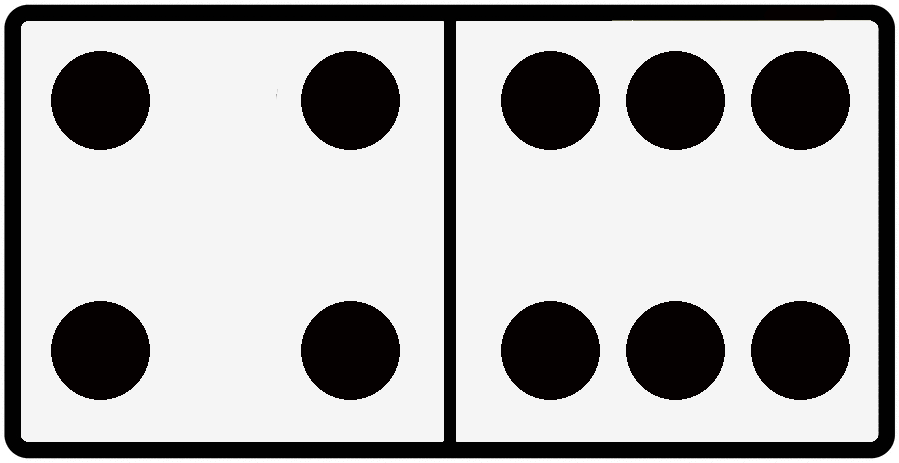
\includegraphics[width=0.2\textwidth]{white4_6.png}}

\footnotesize
(Hint: it's okay to take \textit{zero} of one of the dominoes; \textit{i.e.},
to completely ignore it.)
\normalsize

\item Starter dominoes:
\hspace{.3in}
\raisebox{-0.3\height}{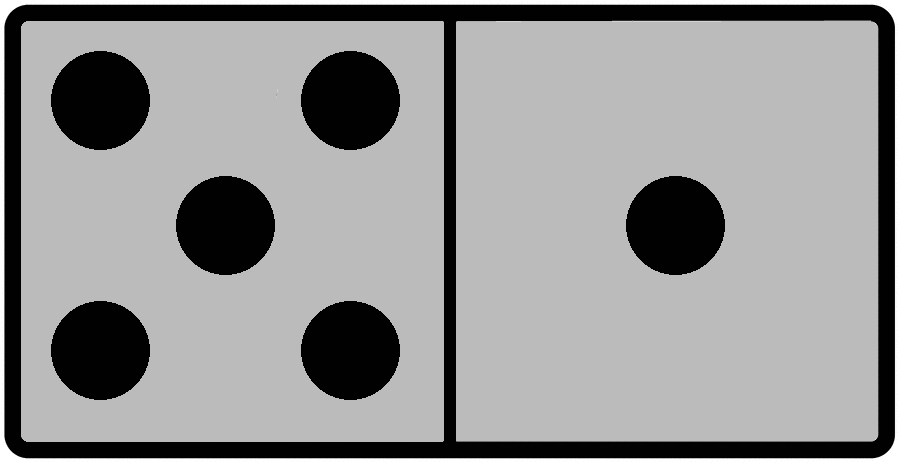
\includegraphics[width=0.2\textwidth]{gray5_1.png}}
\hspace{.1in}
\raisebox{-0.3\height}{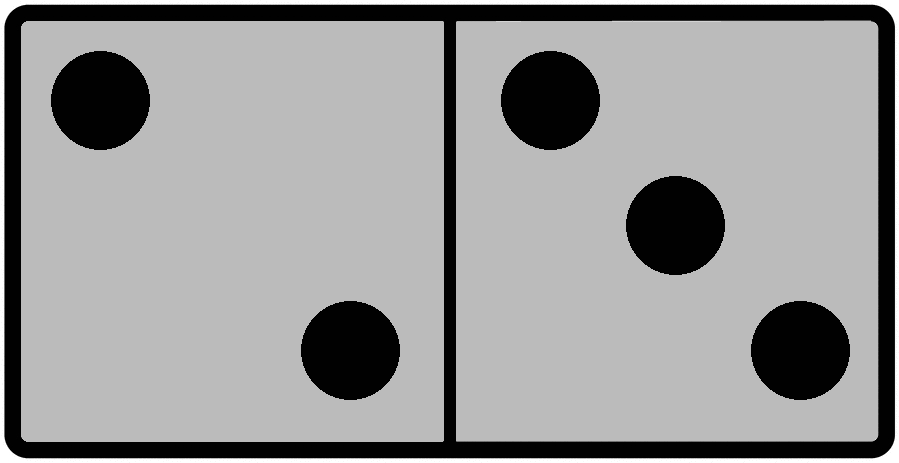
\includegraphics[width=0.2\textwidth]{gray2_3.png}}

Goal domino:
\hspace{1.1in}
\raisebox{-0.3\height}{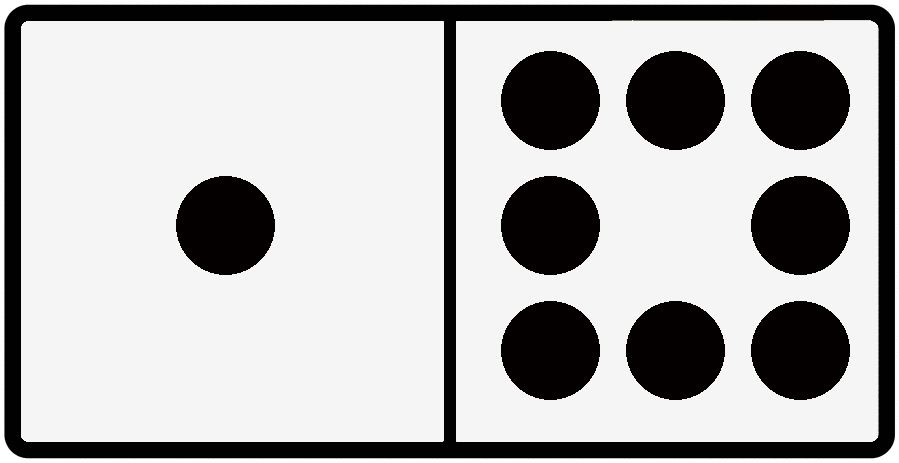
\includegraphics[width=0.2\textwidth]{white1_8.png}}

\footnotesize
(Hint: you may, if you wish, take ``a \textit{negative} number'' of one of the
dominoes. In other words, you can multiply the entire domino by a negative
number and then add it to your multiples of the other one.)
\normalsize

\item Starter dominoes:
\hspace{.3in}
\raisebox{-0.3\height}{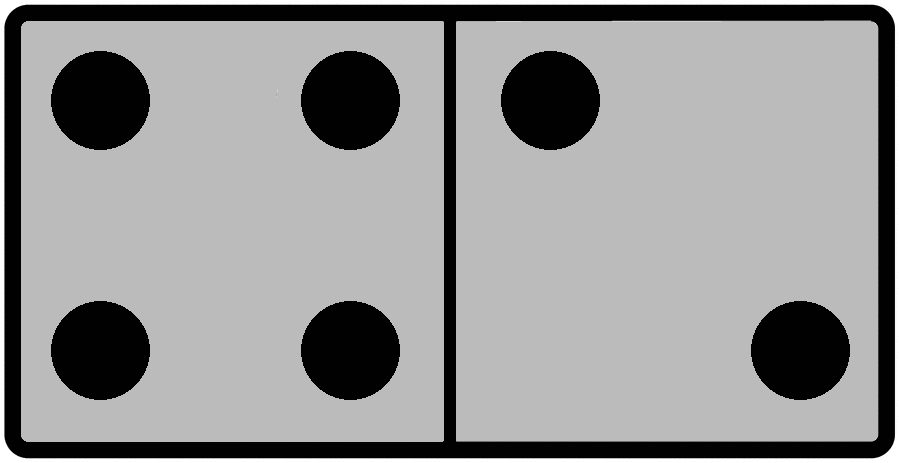
\includegraphics[width=0.2\textwidth]{gray4_2.png}}
\hspace{.1in}
\raisebox{-0.3\height}{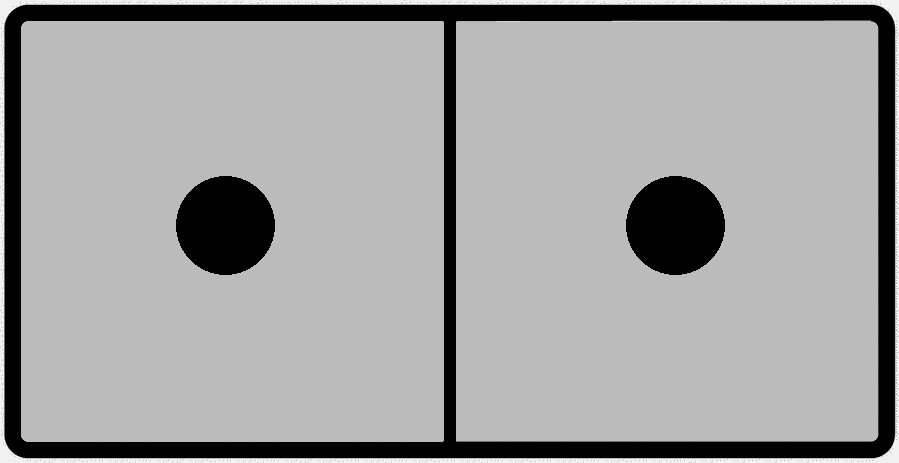
\includegraphics[width=0.2\textwidth]{gray1_1.png}}

Goal domino:
\hspace{1.1in}
\raisebox{-0.3\height}{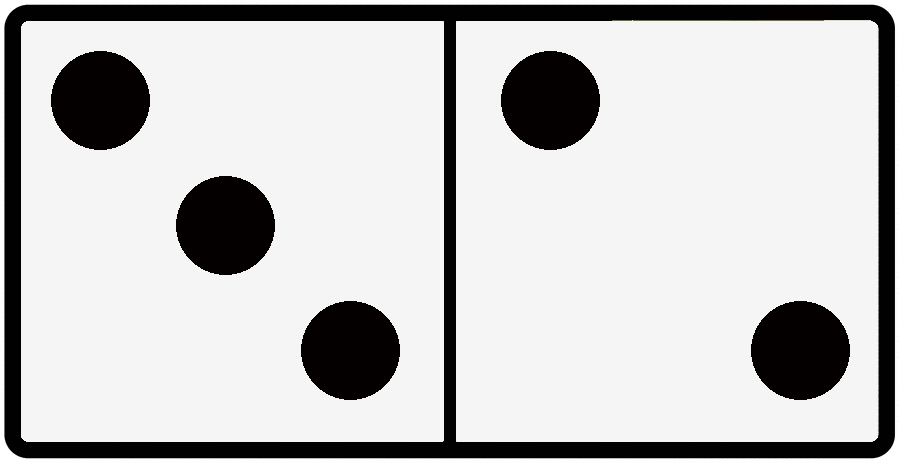
\includegraphics[width=0.2\textwidth]{white3_2.png}}

\footnotesize
(Hint: you can even take a \textit{fraction} of a domino, provided you take the
same fraction of both left and right sides. This means that just as you can
multiply an entire domino by a positive or negative number, or zero, you can
also multiply it by non-integers.)
\normalsize

\pagebreak
\item Starter dominoes:
\hspace{.3in}
\raisebox{-0.3\height}{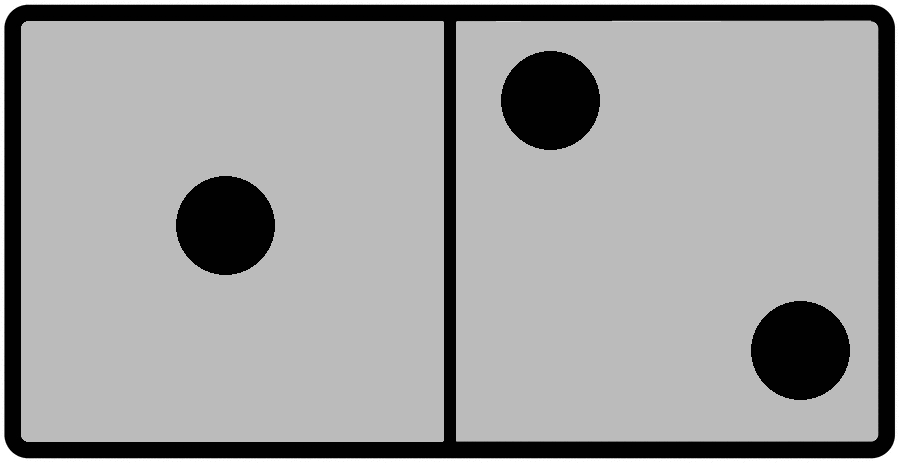
\includegraphics[width=0.2\textwidth]{gray1_2.png}}
\hspace{.1in}
\raisebox{-0.3\height}{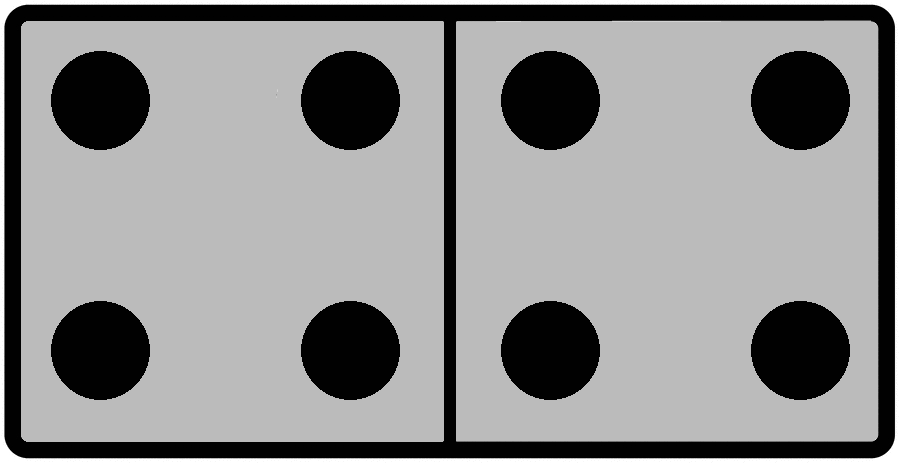
\includegraphics[width=0.2\textwidth]{gray4_4.png}}

Goal domino:
\hspace{1.1in}
\raisebox{-0.3\height}{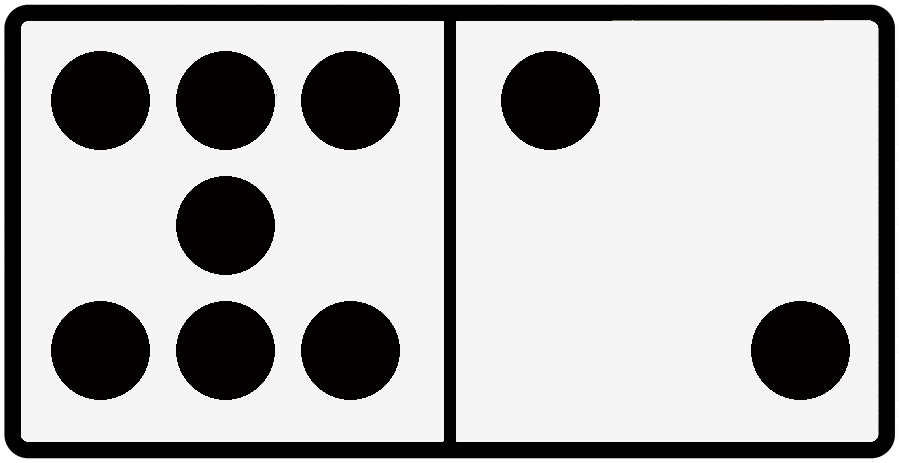
\includegraphics[width=0.2\textwidth]{white7_2.png}}

\footnotesize
(Hint: sometimes you have to go pretty far afield to get a solution, meaning a
large number of one domino and a large \textit{negative} number of the other.)
\normalsize

\item Starter dominoes:
\hspace{.3in}
\raisebox{-0.3\height}{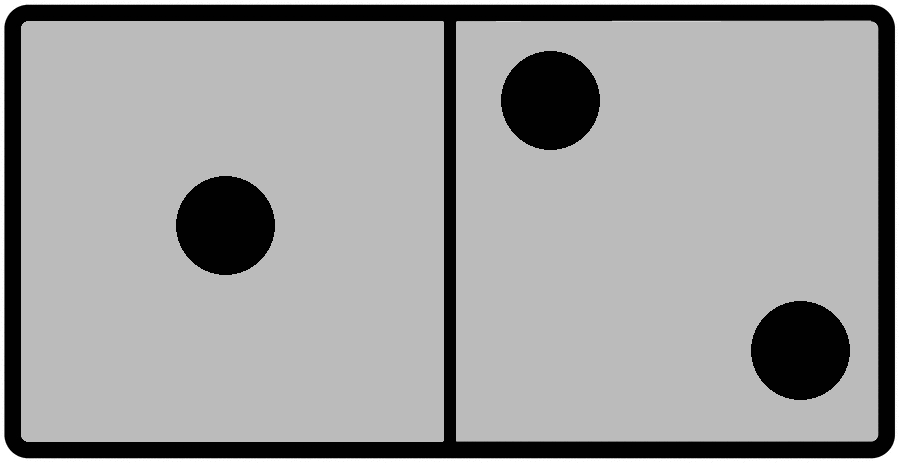
\includegraphics[width=0.2\textwidth]{gray1_2.png}}
\hspace{.1in}
\raisebox{-0.3\height}{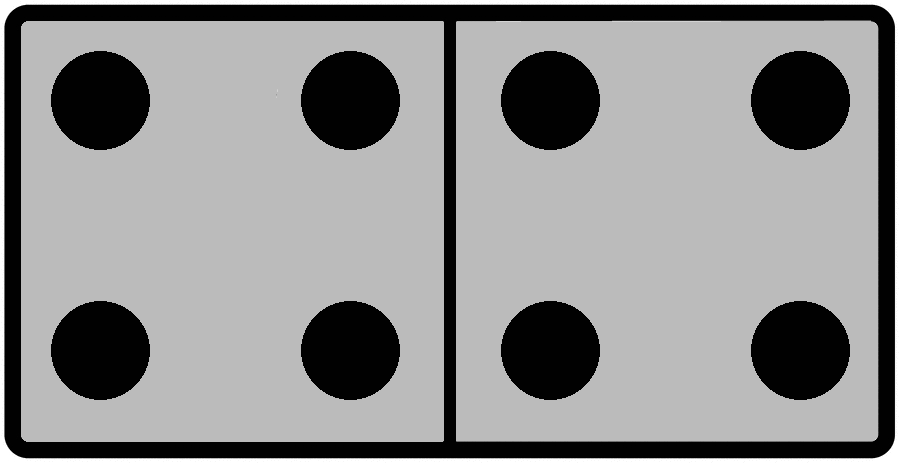
\includegraphics[width=0.2\textwidth]{gray4_4.png}}

Goal domino:
\hspace{1.1in}
\raisebox{-0.3\height}{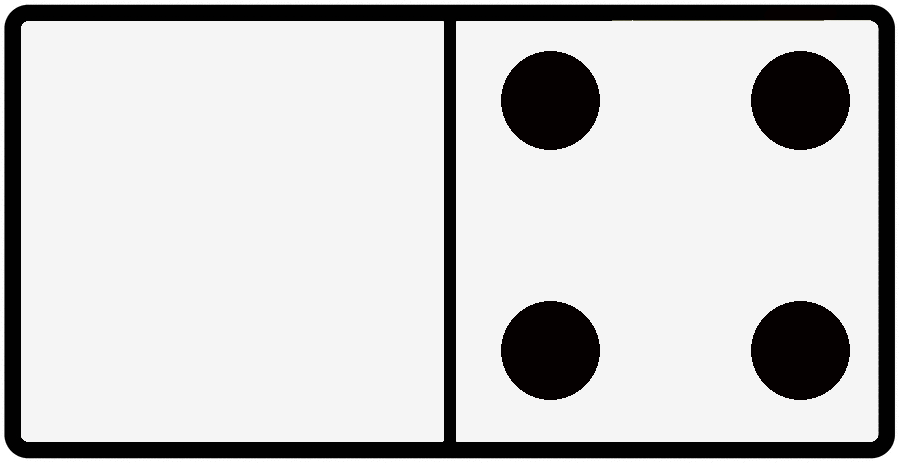
\includegraphics[width=0.2\textwidth]{white0_4.png}}

\footnotesize
(Hint: the goal domino can have a zero on it, just like the starter dominoes
did. But it's really no different; you just have to think creatively about how
to get the numbers to add up to zero on that side.)
\normalsize

\item Starter dominoes:
\hspace{.3in}
\raisebox{-0.3\height}{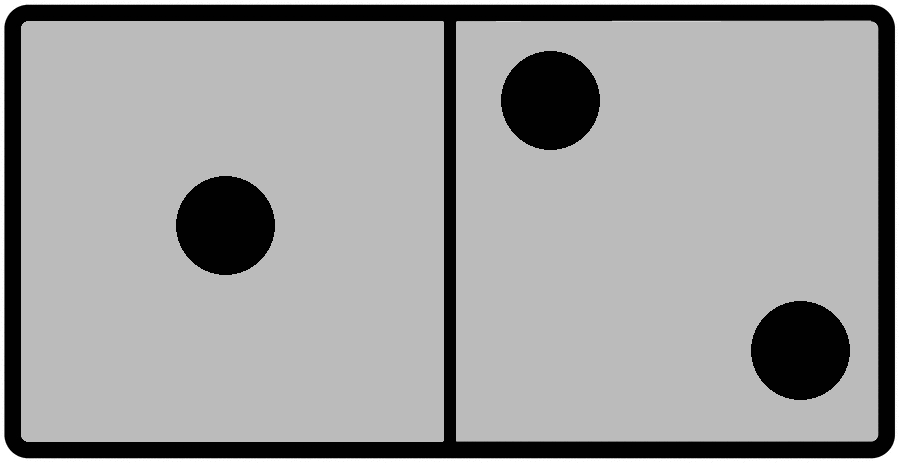
\includegraphics[width=0.2\textwidth]{gray1_2.png}}
\hspace{.1in}
\raisebox{-0.3\height}{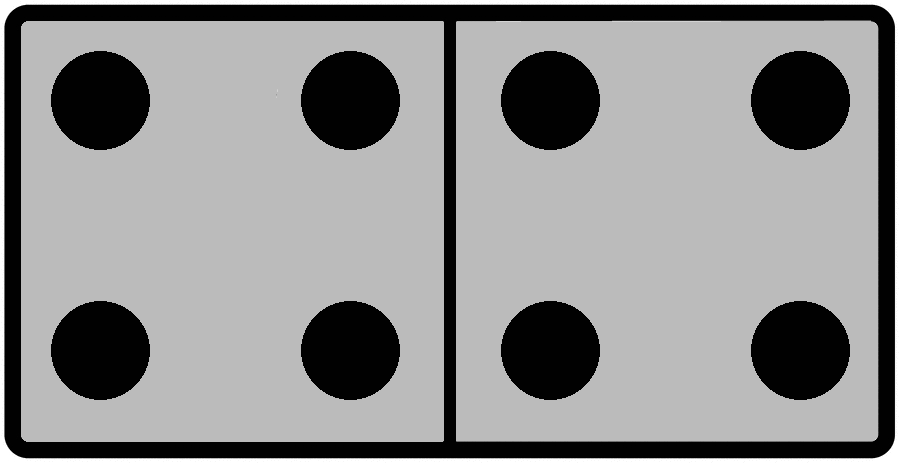
\includegraphics[width=0.2\textwidth]{gray4_4.png}}

Goal domino:
\hspace{1.1in}
\raisebox{-0.3\height}{
\includegraphics[width=0.2\textwidth]{white0_0.png}}

\footnotesize
(Hint: and yeah, the goal domino might even be \textit{completely} zero. That's
really not any different either, and in fact the solution will probably just
jump right off the page at you.)
\normalsize
\label{endDominoPuzzes}
\end{enumerate}

\subsection{Questions for curious minds}

I presume you have tried it, and hopefully succeeded at a few by trial and
error. Even if you didn't, hopefully you looked at and understood the solutions
I gave at the end of the chapter (p.~\pageref{dominoPuzzleAnswers}).

It's well worth taking a moment after all that fiddling around to consider some
interesting questions:

\begin{enumerate}
\itemsep.1em

\item Were your solutions that same as mine in each case? If so, do you think
that was just coincidence? If not, how many different solutions do you think
are possible?

\item Is it always possible to solve a puzzle like this, no matter what the
goal domino is? Or are only a small number of goal dominoes actually possible
to produce?

\item Is it always possible to solve a puzzle like this, no matter what the
starter dominoes are? Or is it only in a few cleverly crafted scenarios where
the numbers happen to work out just right?

\end{enumerate}

We'll shed light on all these matters as we move forward.

\pagebreak
\subsection*{Answers to Domino Game puzzles from
pp.~\pageref{startDominoPuzzes}-\pageref{endDominoPuzzes}}
\label{dominoPuzzleAnswers}

\begin{enumerate}
\itemsep1em

\item {Solution: \textbf{0 \& 2}}

\quad 0 \raisebox{-0.3\height}{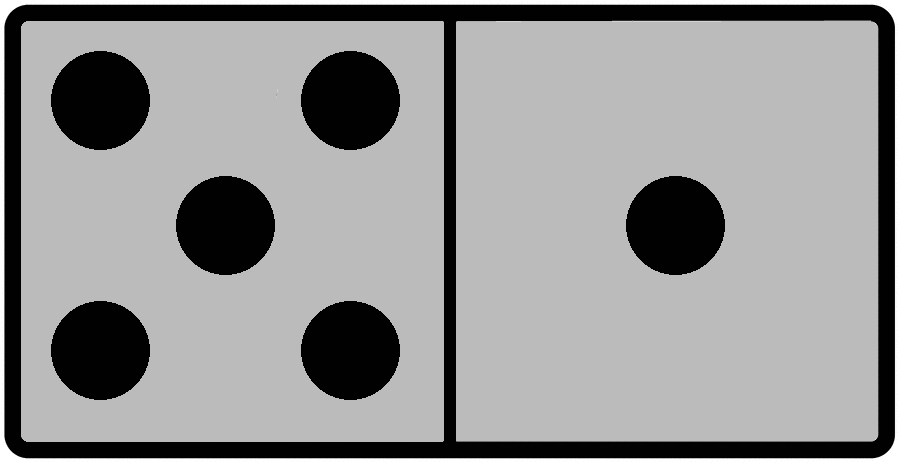
\includegraphics[width=0.1\textwidth]{gray5_1.png}} \ \& \
2 \raisebox{-0.3\height}{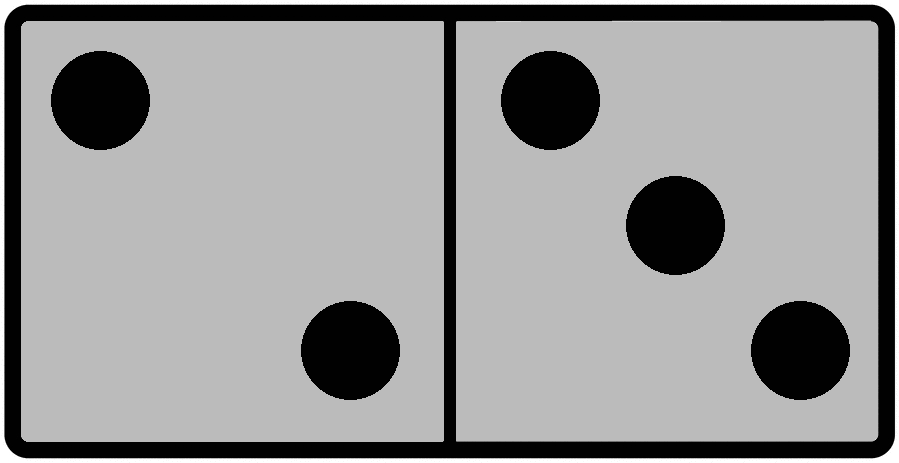
\includegraphics[width=0.1\textwidth]{gray2_3.png}} \ = \
\raisebox{-0.3\height}{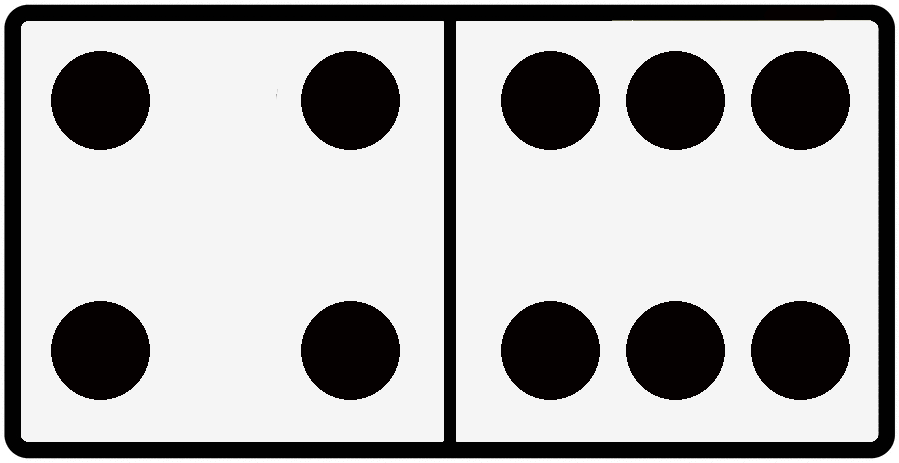
\includegraphics[width=0.1\textwidth]{white4_6.png}} \quad

\item {Solution: \textbf{--1 \& 3}}

\ $-1$ \raisebox{-0.3\height}{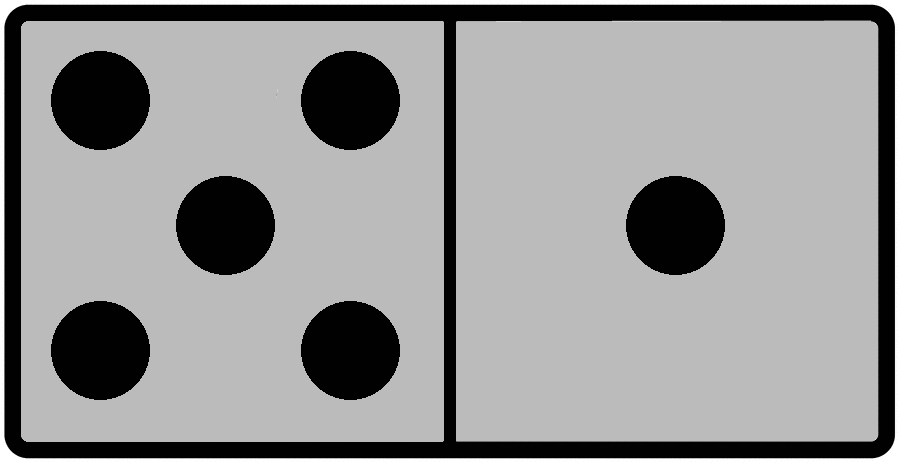
\includegraphics[width=0.1\textwidth]{gray5_1.png}} \ \& \
3 \raisebox{-0.3\height}{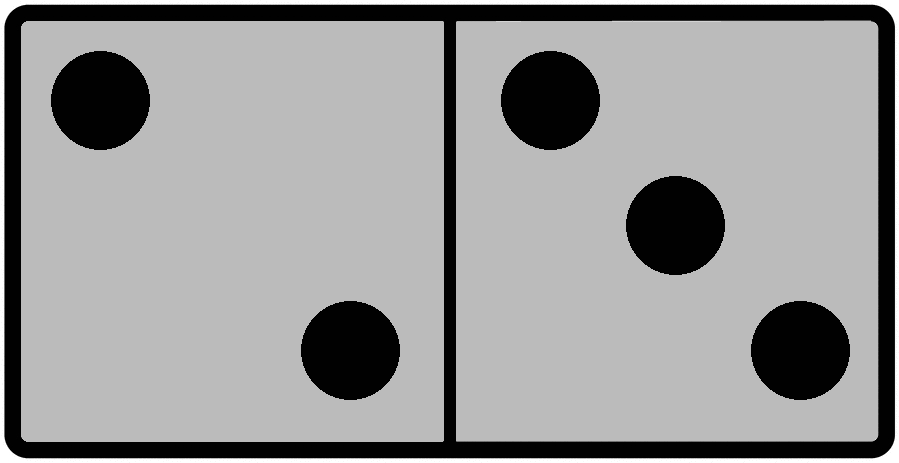
\includegraphics[width=0.1\textwidth]{gray2_3.png}} \ = \
\raisebox{-0.3\height}{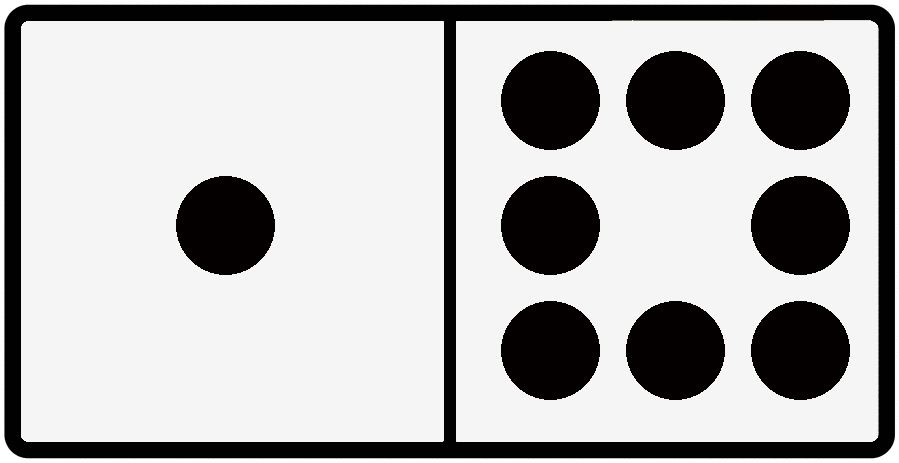
\includegraphics[width=0.1\textwidth]{white1_8.png}} \quad

\item {Solution: \textbf{$\frac{1}{2}$ \& 1}}

\quad $\frac{1}{2}$ \raisebox{-0.3\height}{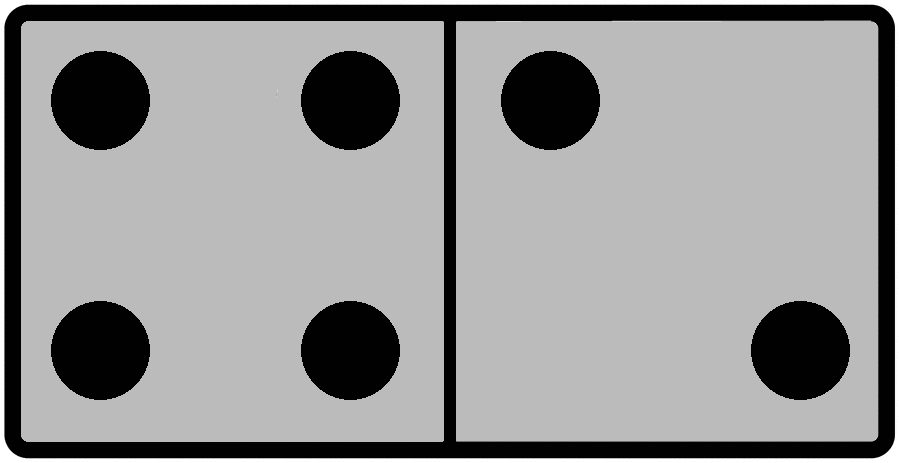
\includegraphics[width=0.1\textwidth]{gray4_2.png}} \ \& \
1 \raisebox{-0.3\height}{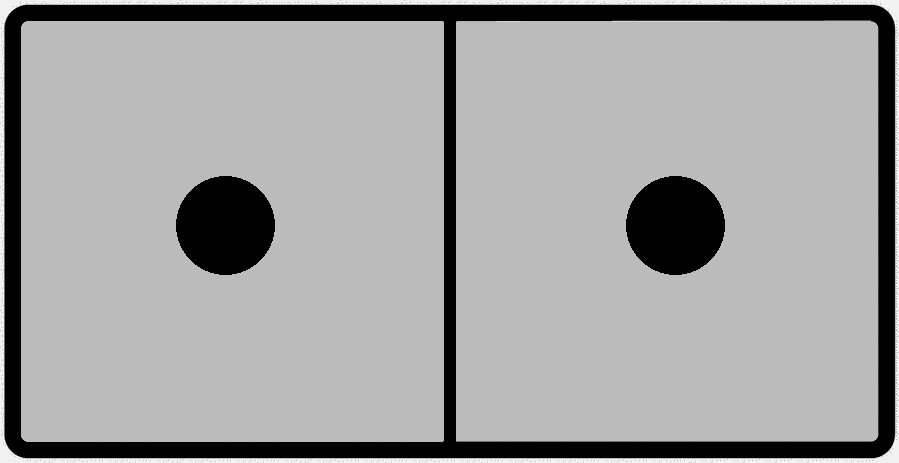
\includegraphics[width=0.1\textwidth]{gray1_1.png}} \ = \
\raisebox{-0.3\height}{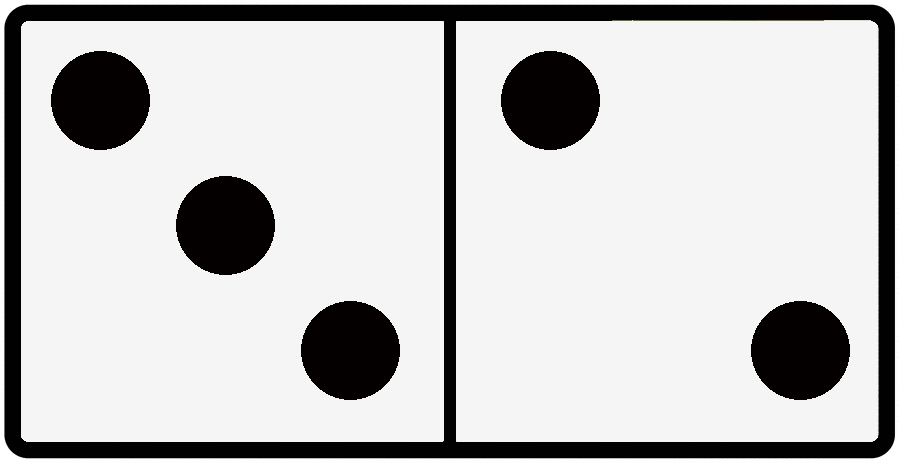
\includegraphics[width=0.1\textwidth]{white3_2.png}} \quad

\item {Solution: \textbf{-5 \& 3}}

\ $-5$ \raisebox{-0.3\height}{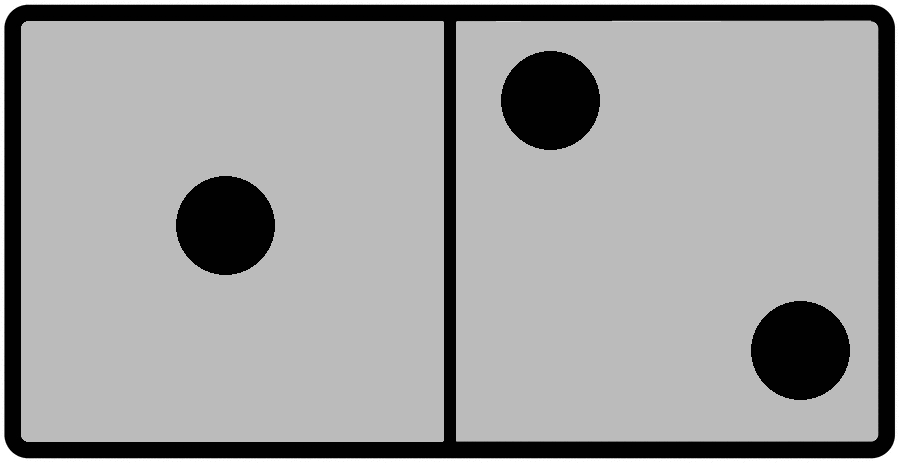
\includegraphics[width=0.1\textwidth]{gray1_2.png}} \ \& \
3 \raisebox{-0.3\height}{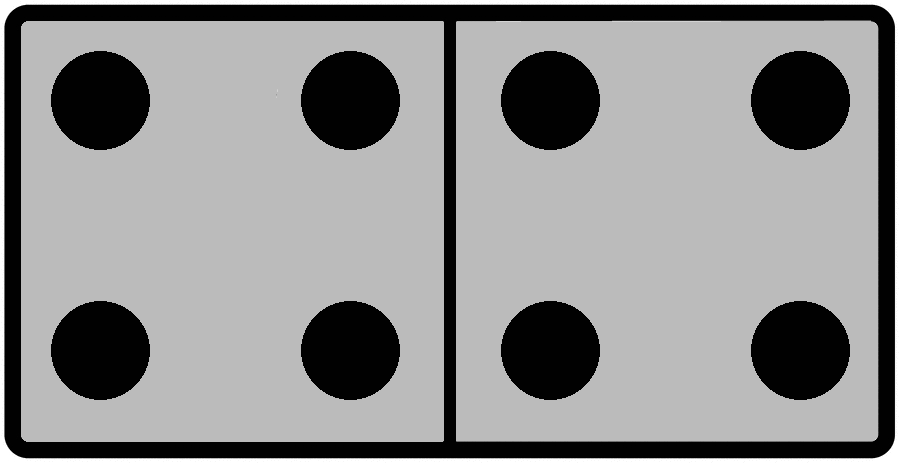
\includegraphics[width=0.1\textwidth]{gray4_4.png}} \ = \
\raisebox{-0.3\height}{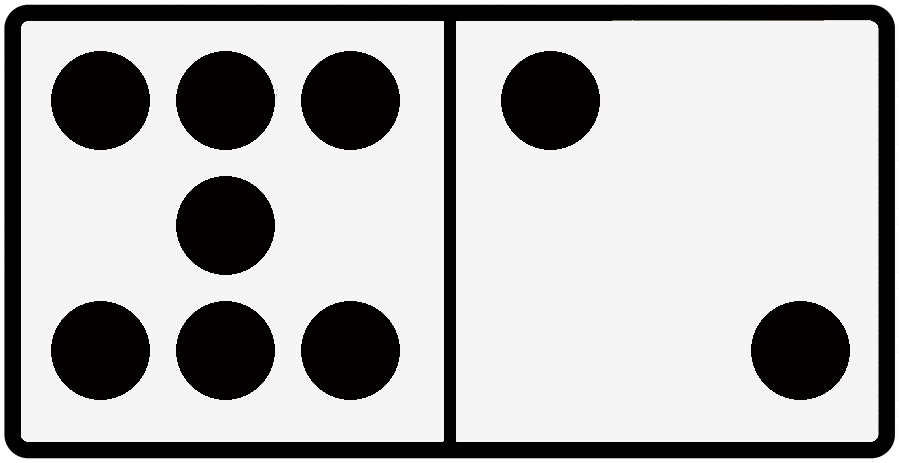
\includegraphics[width=0.1\textwidth]{white7_2.png}} \quad

\item {Solution: \textbf{4 \& --1}}

\quad 4 \raisebox{-0.3\height}{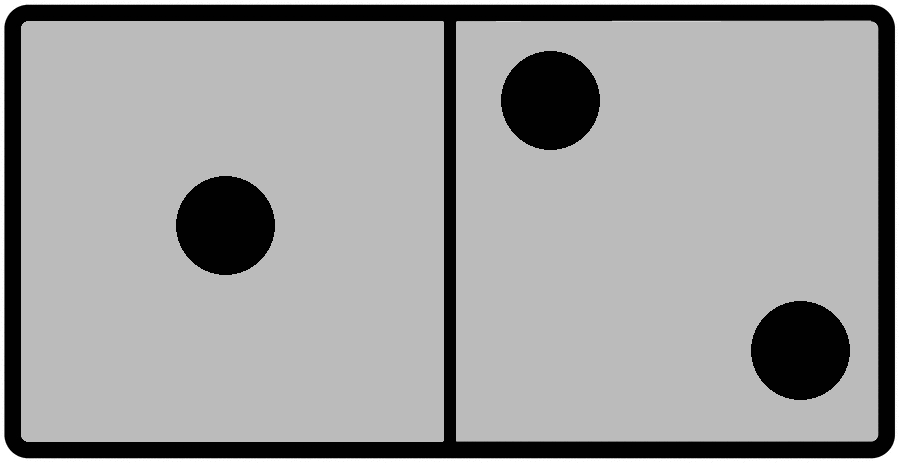
\includegraphics[width=0.1\textwidth]{gray1_2.png}} \&
$-1$ \raisebox{-0.3\height}{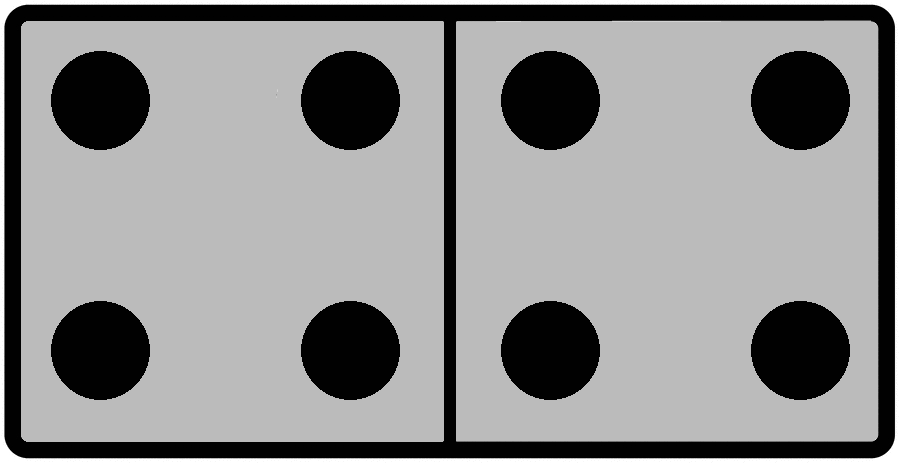
\includegraphics[width=0.1\textwidth]{gray4_4.png}} \ = \
\raisebox{-0.3\height}{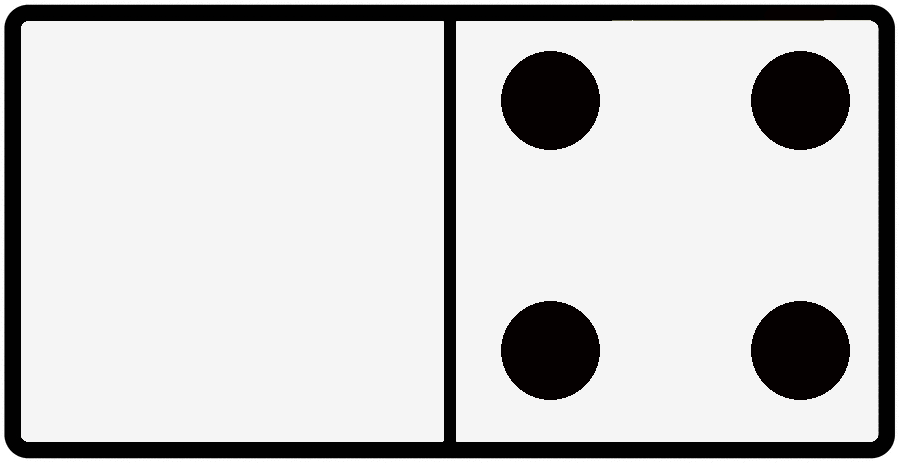
\includegraphics[width=0.1\textwidth]{white0_4.png}} \quad

\item {Solution: \textbf{0 \& 0}}

\quad 0 \raisebox{-0.3\height}{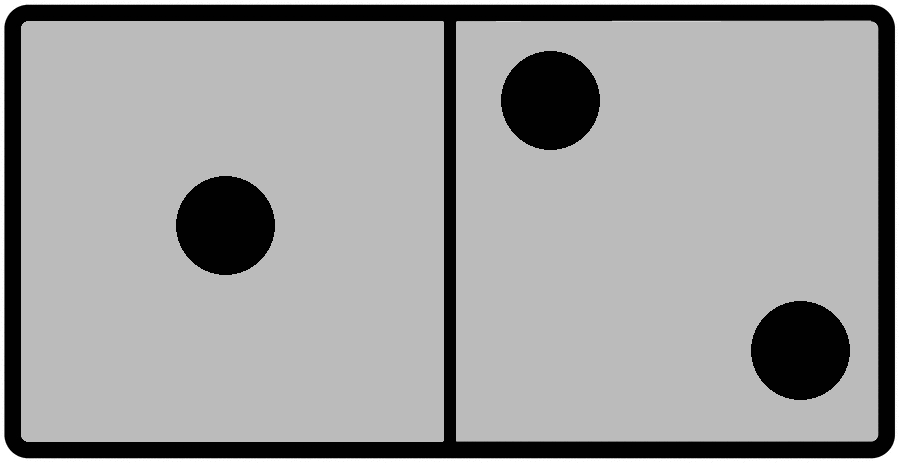
\includegraphics[width=0.1\textwidth]{gray1_2.png}} \ \& \
0 \ \raisebox{-0.3\height}{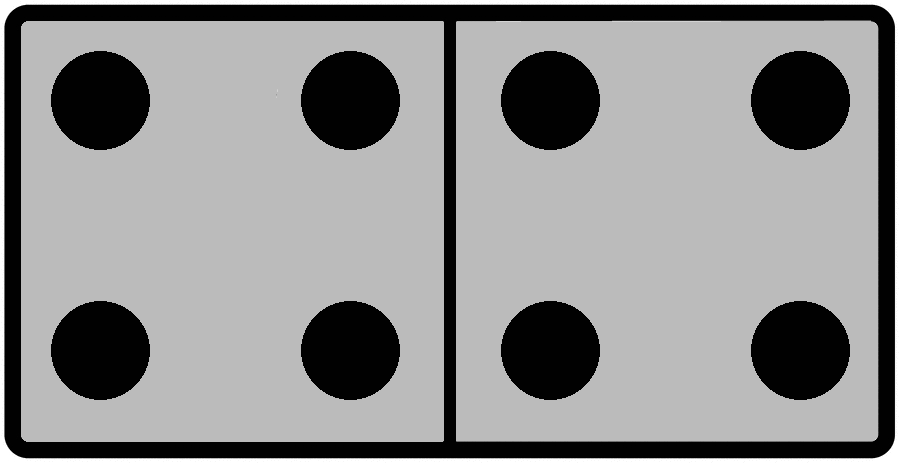
\includegraphics[width=0.1\textwidth]{gray4_4.png}} \ = \
\raisebox{-0.3\height}{
\includegraphics[width=0.1\textwidth]{white0_0.png}} \quad

\end{enumerate}
